\documentclass[tikz,border=2pt]{standalone}
\usepackage{amsmath,amssymb}
\usepackage{pgfplots}
\pgfplotsset{compat=1.18}

\begin{document}
% Density of the standardised mean of n iid Exp(1) observations (a rescaled Gamma(n,1) density)
% for n = 1, 5, 30 against the standard normal density.
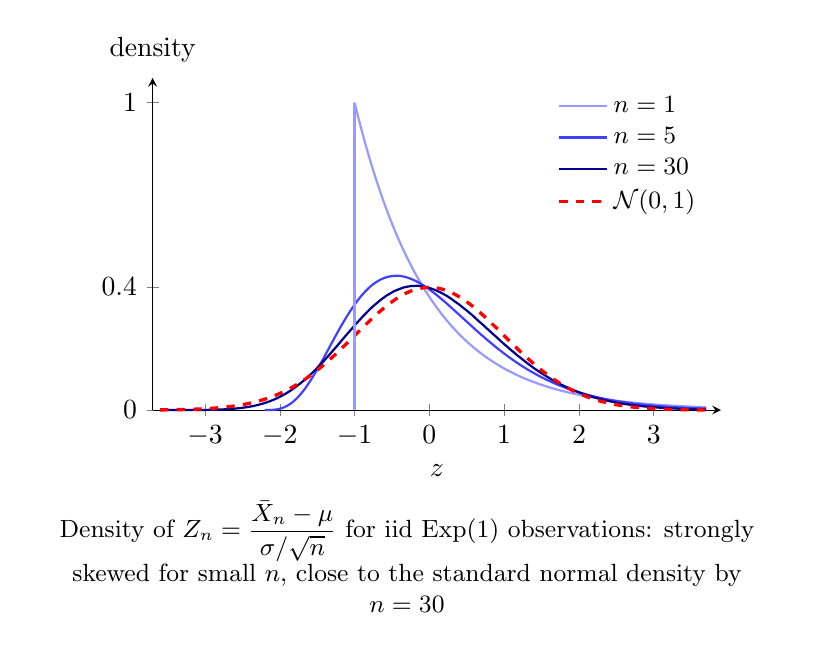
\begin{tikzpicture}
	\begin{axis}[
		axis lines=left, xmin=-3.7, xmax=3.9, ymin=0, ymax=1.08,
		xtick={-3,-2,-1,0,1,2,3}, ytick={0,0.4,1},
		xlabel={$z$}, ylabel={density}, ylabel style={rotate=-90, anchor=south, at={(axis description cs:0,1.02)}},
		samples=160, smooth, width=8.8cm, height=5.8cm, clip=false,
		legend style={draw=none, fill=none, font=\small, at={(0.98,0.98)}, anchor=north east}, legend cell align=left
		]
		\addplot[blue!40, thick, domain=-1:3.7] {exp(-(1+x))};
		\addlegendentry{$n=1$}
		\addplot[blue!75, thick, domain=-2.2:3.7] {sqrt(5)*exp(4*ln(5+sqrt(5)*x)-(5+sqrt(5)*x)-3.178054)};
		\addlegendentry{$n=5$}
		\addplot[blue!55!black, thick, domain=-3.6:3.7] {sqrt(30)*exp(29*ln(30+sqrt(30)*x)-(30+sqrt(30)*x)-71.257039)};
		\addlegendentry{$n=30$}
		\addplot[red, very thick, dashed, domain=-3.6:3.7] {exp(-x^2/2)/sqrt(2*pi)};
		\addlegendentry{$\mathcal{N}(0,1)$}
		\draw[blue!40, thick] (axis cs:-1,0) -- (axis cs:-1,1);
	\end{axis}
	\node[anchor=north, font=\small, align=flush center, text width=9.4cm] at ([yshift=-2pt]current axis.outer south) {Density of $Z_n=\dfrac{\bar X_n-\mu}{\sigma/\sqrt n}$ for iid $\operatorname{Exp}(1)$ observations: strongly skewed for small $n$, close to the standard normal density by $n=30$};
\end{tikzpicture}
\end{document}
